\documentclass[10pt,a4paper]{article}
\usepackage[top=1.4cm, bottom=1.4cm, left=1.6cm, right=1.6cm, headheight=14pt, footskip=18pt]{geometry}
\usepackage[utf8]{inputenc}
\usepackage{amsmath,amsfonts,amssymb}
\usepackage{graphicx}
\usepackage{tikz}
\usepackage{circuitikz}
\usetikzlibrary{calc,patterns}
\usepackage[most]{tcolorbox}
\usepackage{enumitem}
\usepackage{fancyhdr}
\usepackage{booktabs}
\usepackage{tabularx}
\usepackage{colortbl}
\usepackage{hyperref}

% --- Palet Warna Resmi UNIB ---
\definecolor{unibblue}{RGB}{0, 32, 96}
\definecolor{unibgold}{RGB}{197, 160, 89}
\definecolor{unibgreen}{RGB}{34, 112, 60}
\definecolor{boxbg}{RGB}{248, 250, 253}
\definecolor{linegray}{RGB}{210, 215, 225}

% --- Pengaturan Header & Footer ---
\pagestyle{fancy}
\fancyhf{}
\lhead{\footnotesize\textbf{\color{unibblue}Universitas Bengkulu} \textbar\ Program Studi S1 Teknik Elektro}
\rhead{\footnotesize\color{gray}Persamaan Diferensial (Genap 2026)}
\lfoot{\footnotesize\color{gray}Problem Set Tugas Terstruktur Berbasis OBE}
\cfoot{\footnotesize\color{gray}Hal. \thepage\ dari 2}
\rfoot{\footnotesize\color{unibblue}\textbf{Minggu 9: Deret Fourier Trigonometrik \& An...}}
\renewcommand{\headrulewidth}{0.6pt}
\renewcommand{\footrulewidth}{0.4pt}

\begin{document}

% ==================== HALAMAN 1 ====================
\noindent\begin{minipage}[c]{0.68\textwidth}%
  {\large\textbf{\color{unibblue}PROBLEM SET (TUGAS MANDIRI TERSTRUKTUR)}}\\[1mm]
  {\normalsize\textbf{Mata Kuliah: Persamaan Diferensial (2 SKS)}}\\[0.5mm]
  {\small\textbf{Topik Minggu 9:} Deret Fourier Trigonometrik \& Analisis Harmonisa Beban}%
\end{minipage}%
\hfill%
\begin{minipage}[c]{0.30\textwidth}%
  \begin{tcolorbox}[colback=unibblue!5,colframe=unibblue,boxrule=0.6pt,arc=2pt,left=4pt,right=4pt,top=2pt,bottom=2pt]
    \scriptsize
    \textbf{Nama:} \dotfill\\[1.2mm]
    \textbf{NPM:} \dotfill\\[1.2mm]
    \textbf{Kelas/Klp:} \dotfill\\[1.2mm]
    \textbf{Nilai Final:} \hfill \textbf{/ 100}
  \end{tcolorbox}%
\end{minipage}\par

\vspace{1.5mm}

% Kotak Sub-CPMK & Pedoman Tugas Terstruktur
\begin{tcolorbox}[colback=boxbg,colframe=unibgold!90!black,boxrule=0.6pt,arc=2pt,left=5pt,right=5pt,top=3pt,bottom=3pt,title=\textbf{\scriptsize Capaian Pembelajaran (Sub-CPMK 5) \& Pedoman Pengerjaan Tugas}]
  \scriptsize
  \textbf{Sub-CPMK 5:} Mahasiswa mampu menguraikan sinyal periodik non-sinusoidal ke dalam Deret Fourier trigonometrik dan mengevaluasi Total Harmonic Distortion (THD) sesuai standar IEEE Std 519.\\
  \textbf{Ketentuan Tugas:} Kerjakan secara mandiri pada kertas folio/A4 bergaris atau laporan digital rapi. Lampirkan penurunan rumus analitis lengkap dan cetak visualisasi kode program Julia (Soal C6). Kumpulkan pada awal perkuliahan minggu berikutnya.
\end{tcolorbox}

\vspace{1.5mm}

\noindent{\textbf{\color{unibblue}\large BAGIAN I: FONDASI KONSEPTUAL \& PENURUNAN MATEMATIS}}\par
\vspace{1mm}

% Soal C1
\noindent\textbf{1. (C1 - Mengingat \textbar\ Bobot: 10 Poin)}\par\vspace{0.8mm}
{\footnotesize Tuliskan bentuk umum Deret Fourier trigonometrik untuk suatu sinyal periodik $f(t)$ dengan periode $T$ dan frekuensi sudut dasar $\omega_0 = 2\pi/T$, beserta formulasi rumus integral Euler untuk koefisien $a_0$, $a_n$, dan $b_n$.}\par

\vspace{2.5mm}

% Soal C2
\noindent\textbf{2. (C2 - Memahami \textbar\ Bobot: 15 Poin)}\par\vspace{0.8mm}
{\footnotesize Jelaskan mengapa beban non-linier industri (seperti konverter daya thyristor dan Variable Speed Drive) membangkitkan arus harmonisa pada sistem tenaga listrik. Bagaimana deret Fourier memisahkan komponen fundamental dari distorsi harmonisa?}\par

\vspace{2.5mm}

% Soal C3
\noindent\textbf{3. (C3 - Menerapkan \textbar\ Bobot: 20 Poin)}\par\vspace{0.8mm}
\noindent\begin{minipage}[t]{0.60\textwidth}%
  {\footnotesize Tinjau arus beban penyearah gelombang penuh satu fasa tanpa filter yang menghasilkan gelombang pulsa persegi terpotong periodik pada gambar di samping dengan periode $T=20\text{ ms}$ ($f_0 = 50\text{ Hz}$) dan amplitudo puncak $I_m = 30\text{ A}$. Turunkan koefisien deret Fourier $a_0$, $a_n$, dan $b_n$ secara analitis!}%
\end{minipage}%
\hfill%
\begin{minipage}[t]{0.37\textwidth}%
  \centering
  \resizebox{0.95\linewidth}{!}{%
  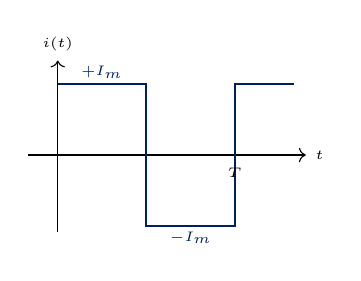
\begin{tikzpicture}[scale=0.75]
    \draw[->] (-0.5,0) -- (4.2,0) node[right, font=\tiny] {$t$};
    \draw[->] (0,-1.3) -- (0,1.6) node[above, font=\tiny] {$i(t)$};
    \draw[thick, unibblue] (0,1.2) -- (1.5,1.2) -- (1.5,-1.2) -- (3.0,-1.2) -- (3.0,1.2) -- (4.0,1.2);
    \node at (0.75,1.4) [font=\tiny\bfseries, unibblue] {$+I_m$};
    \node at (2.25,-1.4) [font=\tiny\bfseries, unibblue] {$-I_m$};
    \node at (3.0,-0.3) [font=\tiny] {$T$};
  \end{tikzpicture}%
  }%
\end{minipage}\par

\vfill

% Kotak Formula Rujukan Teknis & Standar Industri
\begin{tcolorbox}[colback=unibblue!3,colframe=unibblue,colbacktitle=unibblue,coltitle=white,boxrule=0.6pt,arc=2pt,left=6pt,right=6pt,top=3pt,bottom=3pt,title=\textbf{\scriptsize FORMULA RUJUKAN TEKNIS \& STANDAR INDUSTRI TERKAIT}]
  \scriptsize
  \begin{itemize}[leftmargin=*, nosep]
  \item Deret Fourier Trigonometrik: $f(t) = a_0 + \sum_{n=1}^\infty \left( a_n \cos(n\omega_0 t) + b_n \sin(n\omega_0 t) \right)$
  \item Koefisien Euler: $a_0 = \frac{1}{T}\int_0^T f(t) dt$, $a_n = \frac{2}{T}\int_0^T f(t)\cos(n\omega_0 t) dt$, $b_n = \frac{2}{T}\int_0^T f(t)\sin(n\omega_0 t) dt$
  \item Standar Batas Harmonisa \textbf{IEEE Std 519}: Batas Total Harmonic Distortion Arus $\text{THD}_i \le 5{,}0\%$
  \item Formulasi THD: $\text{THD}_i = \frac{\sqrt{\sum_{n=2}^\infty I_n^2}}{I_1} \times 100\%$
\end{itemize}
\end{tcolorbox}

\newpage
% ==================== HALAMAN 2 ====================

\noindent{\textbf{\color{unibblue}\large BAGIAN II: ANALISIS SISTEM, EVALUASI STANDAR, \& KOMPUTASI JULIA}}\par
\vspace{1mm}

% Soal C4
\noindent\textbf{4. (C4 - Menganalisis \textbar\ Bobot: 20 Poin)}\par\vspace{0.8mm}
{\footnotesize Berdasarkan deret Fourier arus Soal 3: (a) Hitung amplitudo komponen harmonisa ke-1 ($I_1$), ke-3 ($I_3$), dan ke-5 ($I_5$); (b) Hitung Total Harmonic Distortion arus ($\text{THD}_i$) menggunakan 5 suku harmonisa pertama; (c) Analisis apakah nilai $\text{THD}_i$ tersebut memenuhi ambang batas standar \textbf{IEEE Std 519} (maksimal $5{,}0\%$).}\par

\vspace{3.5mm}

% Soal C5
\noindent\textbf{5. (C5 - Mengevaluasi \textbar\ Bobot: 20 Poin)}\par\vspace{0.8mm}
{\footnotesize Suatu sistem tenaga menyuplai tegangan sinusoidal murni $v(t) = 311 \cos(100\pi t)\text{ V}$ ke beban non-linier yang menarik arus terdistorsi $i(t) = 15 \cos(100\pi t - 30^\circ) + 5 \cos(300\pi t - 45^\circ) + 2 \cos(500\pi t - 60^\circ)\text{ A}$. Evaluasi daya aktif total ($P$), daya distorsi ($D$), dan faktor daya sejati (*true power factor*) sistem!}\par

\vspace{3.5mm}

% Soal C6
\noindent\textbf{6. (C6 - Merancang \& Komputasi Julia \textbar\ Bobot: 15 Poin)}\par\vspace{0.8mm}
{\footnotesize Rancang skrip program ilmiah dalam bahasa \textbf{Julia} untuk merekonstruksi gelombang arus persegi Soal 3 melalui penjumlahan $N$ harmonisa pertama Deret Fourier. Program harus memplot perbandingan kurva rekonstruksi untuk $N \in \{1, 3, 7, 25\}$ dan menunjukkan fenomena overshoot Gibbs di dekat titik diskontinuitas.}\par

\vfill

% Tabel Rekapitulasi Skor OBE & Lembar Catatan Umpan Balik Dosen
\noindent\begin{minipage}[b]{0.62\textwidth}%
  \centering
  \scriptsize
  \begin{tabular}{|c|c|c|c|c|c|c|}
    \hline
    \rowcolor{unibblue}
    \textbf{\color{white}C1} & \textbf{\color{white}C2} & \textbf{\color{white}C3} & \textbf{\color{white}C4} & \textbf{\color{white}C5} & \textbf{\color{white}C6} & \textbf{\color{white}Total} \\
    \rowcolor{unibblue!10}
    10 Pts & 15 Pts & 20 Pts & 20 Pts & 20 Pts & 15 Pts & 100 Pts \\
    \hline
    & & & & & & \\[3mm]
    \hline
  \end{tabular}%
\end{minipage}%
\hfill%
\begin{minipage}[b]{0.35\textwidth}%
  \centering
  \scriptsize
  \textbf{Verifikasi Dosen / Asisten:}\\[6mm]
  (\dotfill)\\[1mm]
  \tiny Tanggal: \dotfill
\end{minipage}\par

\vspace{2mm}
\begin{tcolorbox}[colback=white,colframe=unibblue!40!black,colbacktitle=unibblue!10,coltitle=unibblue,boxrule=0.5pt,arc=2pt,left=5pt,right=5pt,top=3pt,bottom=3pt,title=\textbf{\tiny Catatan Evaluasi \& Umpan Balik Dosen Pengampu}]
  \tiny
  \textbf{Rubrik Pemeriksaan Pengerjaan Tugas Mandiri:}\par\vspace{0.8mm}
  $\square$ Penurunan matematis langkah-demi-langkah runtut (C1--C4) \hfill $\square$ Validasi analitis \& standar industri IEEE/IEC/SPLN akurat (C5)\\[0.8mm]
  $\square$ Skrip program Julia mandiri \& grafik visualisasi terlampir (C6) \hfill $\square$ Kerapian format laporan \& ketepatan waktu pengumpulan\\[2.0mm]
  \textbf{Catatan / Koreksi Khusus Dosen:}\\[1.6cm]
\end{tcolorbox}

\end{document}
